\section{Top-Level Forms}

\mbox{PyPltRedex supports three primary forms. \texttt{define-language} and \texttt{define-metafunction}} forms are lifted directly PLTRedex. \texttt{reduction-relation} form had to be modified resulting in \texttt{define-reduction-relation}. \texttt{read-from-stdin-and-apply-reduction-relation*} form  is based on  \texttt{apply-reduction-relation} but instead it reads a term from standard input, parses it, and only then applies reduction relation. The grammar for these forms can be found in Figure \ref{grammar-tlmain}.

\begin{figure}
\begin{minted}[tabsize=2,obeytabs,escapeinside=//,mathescape=true,fontsize=\normalsize]{text}
define-language = ( define-language language-name non-terminal-definition+ )
non-terminal-definition = ( non-terminal-name ::= pattern+ )

define-metafunction = ( define-metafunction language-name metafunction-contract metafunction-case+ )
metafunction-contract =	id : pattern-sequence* -> pattern
metafunction-case =  [( name pattern* ) term-template]

reduction-relation = ( define-reduction-relation name language domain reduction-case+ )
reduction-case = (-> pattern term-template reduction-case-name)
domain = #:domain pattern

read-from-stdin-and-apply-reduction-relation = ( read-from-stdin-and-apply-reduction-relation :#mf metafunction-name )
\end{minted}
\caption{Grammar for primary top-level forms.}
\label{grammar-tlmain}
\end{figure}

\begin{itemize}
\item
\TlDefineLanguage. $n$ is the name of the language and $nt_1,...,nt_m$ are \NtDefinitionN \space instances containing one or more \texttt{Pattern} instances.

\item
\TlDefineMetafunction. $n$ is the \texttt{id} specified by \texttt{metafunction-contract}. Let $p_1, ..., p_n$ be the pattern sequence specified by the \texttt{metafunction-contract}, between \texttt{id} and \texttt{->}. $domain$ pattern is then constructed in the following way: \mintinline{text}{PatternSequence(|$n$|, [|$p_1$|, |$...$|, |$p_n$|])}. $codomain$ pattern is the one following \texttt{->}. If input term doesn't match pattern $domain$, an Exception is raised. Similarly, if the resulting term doesn't match $codomain$ pattern, an Exception is also raised. If metafunction produces no terms, an Exception is raised. $mc_1,...,mc_n$ is the sequence of \space \MetafunctionCase \space containing the pattern $p$ to be matched and the term-template $t$ to plug matches into. $l$ is the name of the language with respect to which all non-terminal symbols in patterns $p$ are resolved.

\item \TlDefineReductionRelation. $n$ is the name of the reduction-relation; an optional $domain$ pattern ensures that the input term and resulting terms match the pattern otherwise an Exception is raised, and each $rc_i$=\ReductionCase \space contains a pattern $p$ and term-template $t$; $n$ is the name of the reduction case.

This form had to be modified due to the fact that PyPltRedex doesn't interpret Racket in any way and thus \texttt{define} form is not supported. Therefore, \texttt{define} and \texttt{reduction-relation} forms had to be collapsed into a single \texttt{define-reduction-relation} form.

\item \ReadFromStdinAndApplyReductionRelation \space is self-explanatory -  it reads a string from a standard input or file, parses it into a term using logic outlined in Section \ref{section:lex-parse}, and applies a reduction-relation with name $r$. Optionally, one can provide the metafunction with a name $f$ to apply to the parsed term before application of $r$. This allows for separation of the specification of "code" from everything else that is required to evaluate the "code" (such as model of the heap/stack, etc).
\end{itemize}

PyPltRedex provides several additional forms with testing functionality. The goal is to run individual components of PyPltRedex, such as the pattern matcher and term generator, and then compare the results against expected ones. These additional forms are \texttt{redex-match-assert-equal}, \texttt{term-let-assert-equal} and \\ \texttt{apply-reduction-relation-assert-equal}.

\begin{itemize}
\item \RedexMatchAssertEqual. Given a term instantiated from term-template $t$, it is matched against a pattern $p$ containing non-terminal symbols from language $l$. A resulting list of matches is then compared against the list of expected matches $m_1,...,m_n$, potentially empty, where $m_i=$\space\Match. The term instantiated from term-template $t_i$ is assigned to pattern-variable $s_i$. An Exception is raised under the following conditions:
	\begin{enumerate}
	\item Lengths of both lists do not match.
	\item Given two matches from both lists at position $i$, $m_i^{expected} \neq m_i^{actual}$, with the equality operation defined in Section \ref{section:Match}.
	\end{enumerate}
	This form is based on the \texttt{redex-match} form provided by PLTRedex.

\item \TermLetAssertEqual. Given a list of pattern-variable assignments $(v_i, n_i, t_i)$, a new \texttt{Match} instance is created, the term instantiated from the term-template $t_i$ is assigned to the pattern-variable $v_i$. The resulting \texttt{Match} is then plugged into term-template $t$, and the resulting term is compared against a term produced by term-template $e$.

\item \ApplyReductionRelationAssertEqual. This form takes a term produced by the term-template $t$, applies reduction relation with name $r$, and then compares resulting terms against a list of terms instantiated from term-templates $e_1,...,e_n$.
	\begin{enumerate}
	\item Lengths of both lists do not match.
	\item Given two terms from both lists at position $i$, $t_i^{expected} \neq t_i^{actual}$, with equality operation defined in Section \ref{section:runtime-terms}
	\end{enumerate}
\end{itemize}

Figure \ref{class-diagram-toplevel} shows class diagram for all top-level forms.

\begin{figure}[htb]
	\centering
	\makebox[\textwidth][c] { 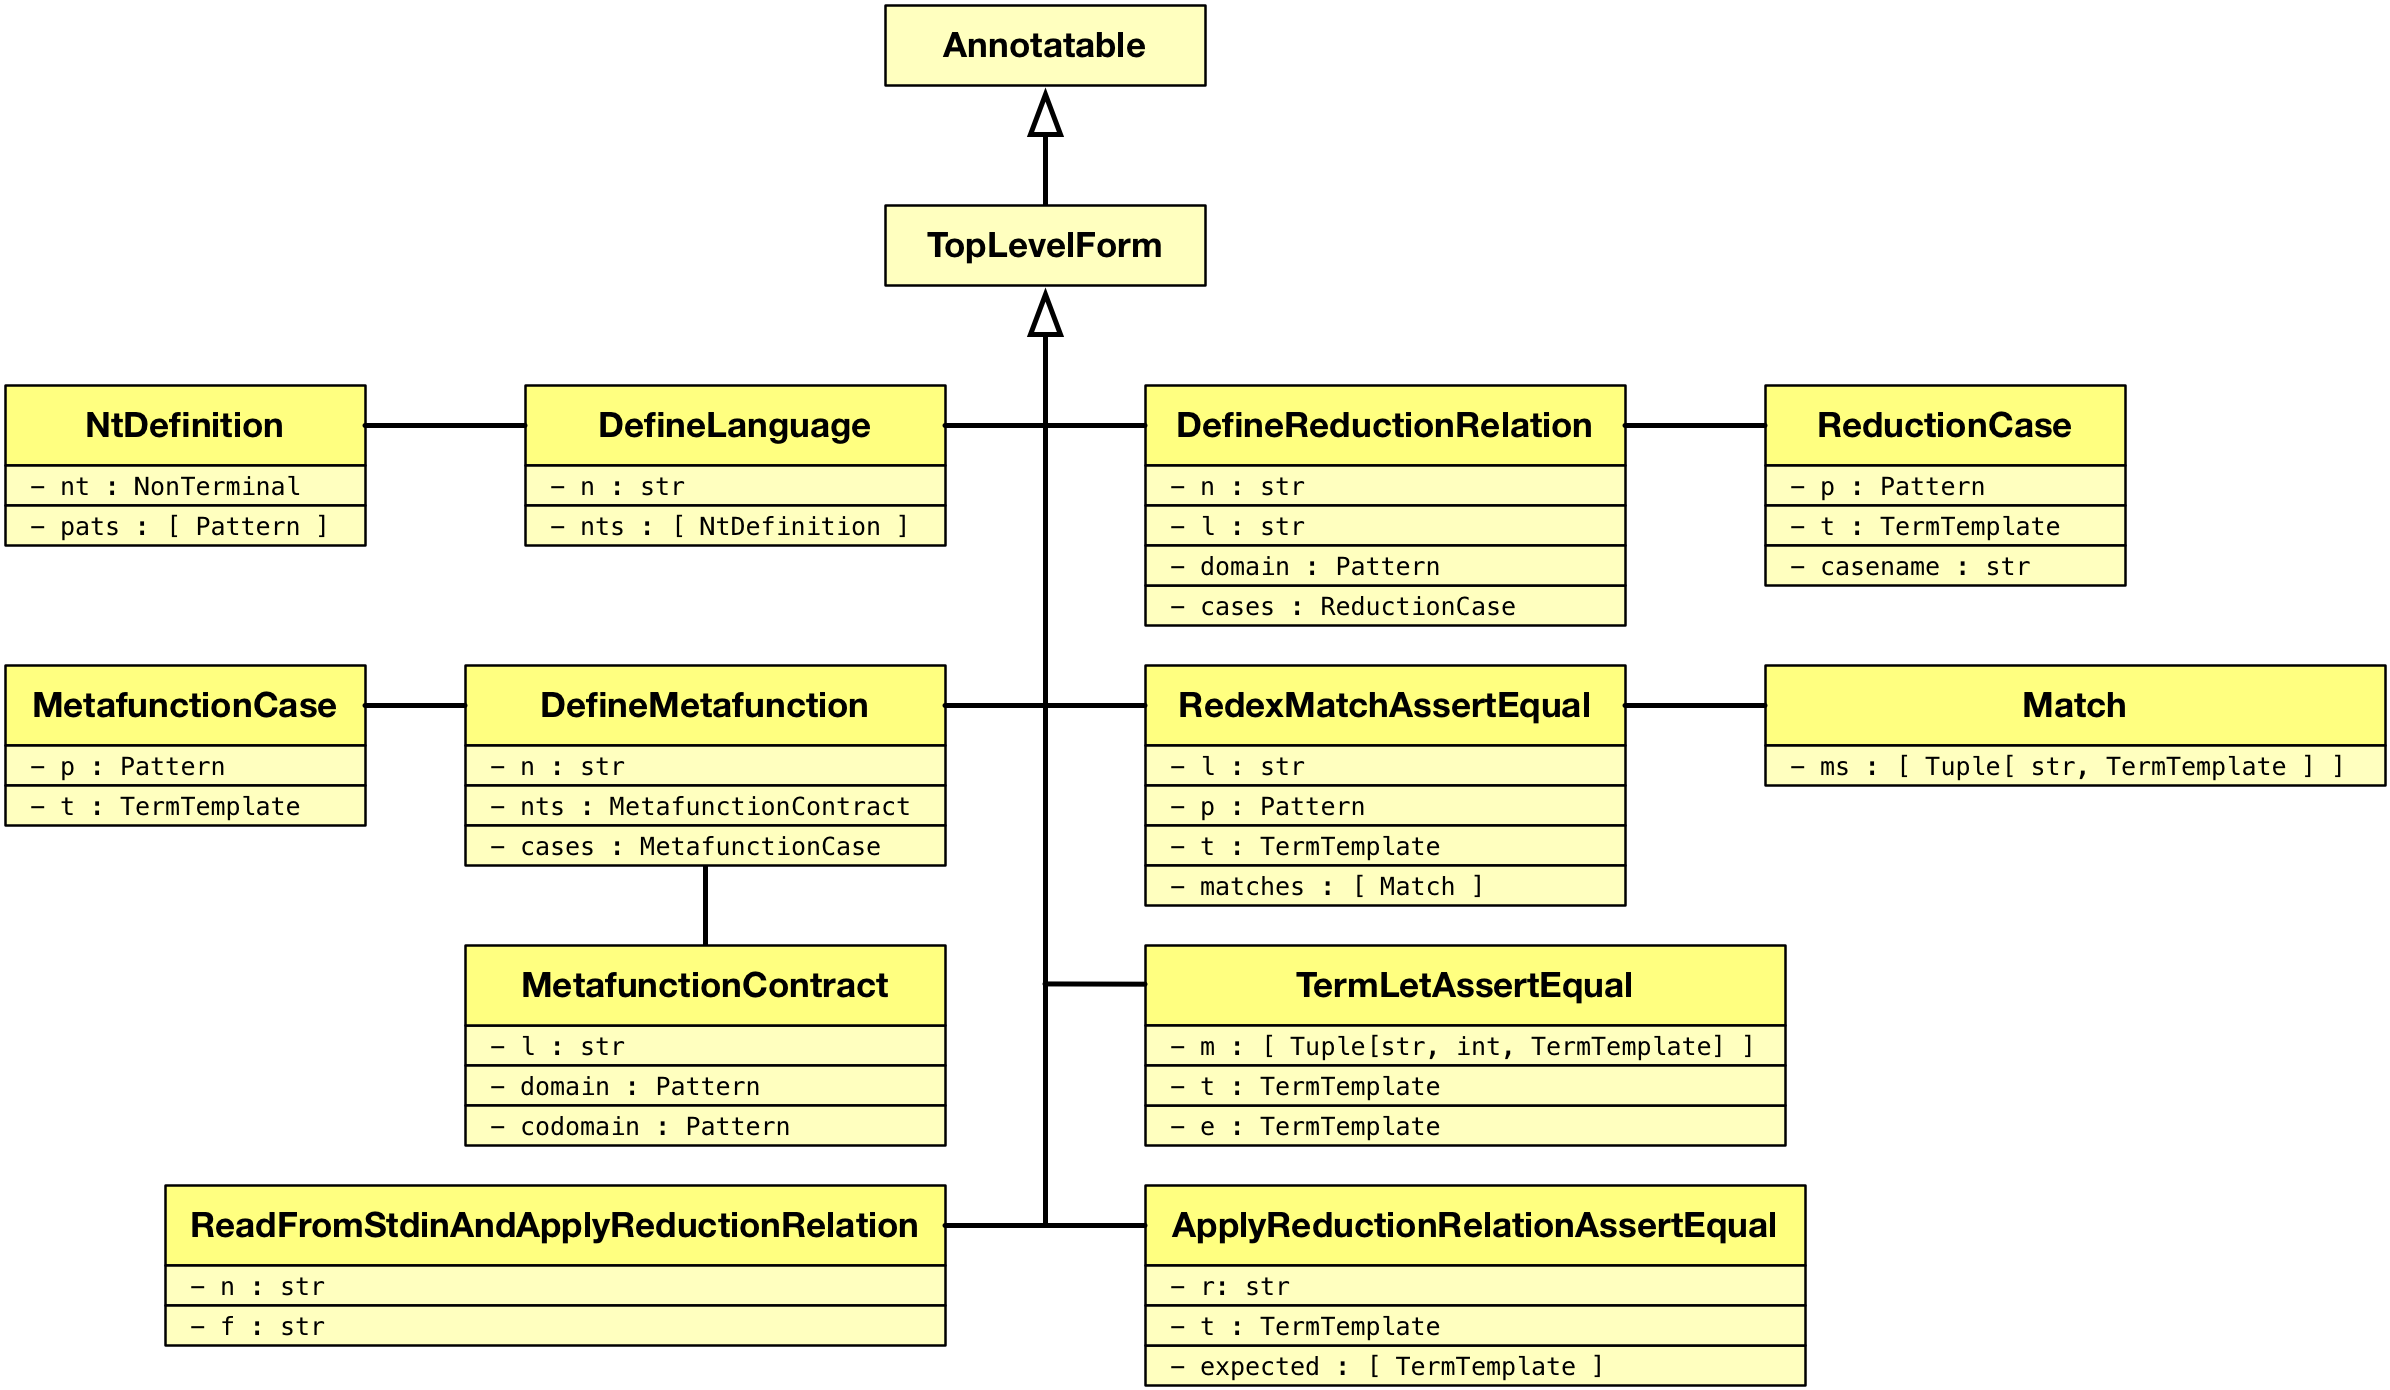
\includegraphics[scale=0.21]{class-diagram-toplevel.png} }
	\caption{Representation of top-level forms.}
\label{class-diagram-toplevel}
\end{figure}
